%!TEX root = ../thesis.tex
\chapter{Yauhau}

\label{ch:Yauhau}

\yauhau{} is a plugin for the Ohua compiler.
It was first introduced in the paper ``Ÿauhau: Concise Code and Efficient I/O Straight from Dataflow.''~\cite{ErtelGoensAdamEtAl2016}, where a more detailed account of the motivation, implementation and results may be found.
Following I will briefly outline the basic transformation in \yauhau{} which is necessary to understand the arising problems which I am solving in the Chapters following.

\yauhau{} hooks into the compiler after the Clojure source has been parsed and transformed into the dataflow IR.
It is a pure IR to IR transformation.
In the flow graph in Figure~\ref{fig:ohua-compiler-flow} \yauhau{} would be run as part of the IR optimisation step.
Additionally a map of context information is given to the plugin.
The precise nature of this context information will be explained in section \ref{ch:Context} its information is used in the transformations of Chapter~\ref{ch:if-transformation} and Chapter~\ref{ch:smap-transformation}.
It is irrelevant to the basic \yauhau{} idea and transformation.

Fundamentally \yauhau{} performs a graph transformation on the dataflow graph it has been given in form of the IR.
The goal behind this transformation is to find sets of I/O operations which are data independent from each other.
This is functionally similar to the approach taken by Haxl\cite{Haxl:library:link}, see Chapter~\ref{ch:related-work}.
Haxl leverages the Monad and Applicative abstractions provided by the Haskell language and base library to propagate a list of parallel executable I/O actions through the program path, blocking each path as soon as an I/O action is encountered.
This is a dynamic way of finding parallel I/O actions, i.e. at runtime a data structure (Data.Sequence.Seq) is populated with pending requests.
\yauhau{} takes a different approach and statically finds parallel I/O actions at compile time.

\begin{figure}
    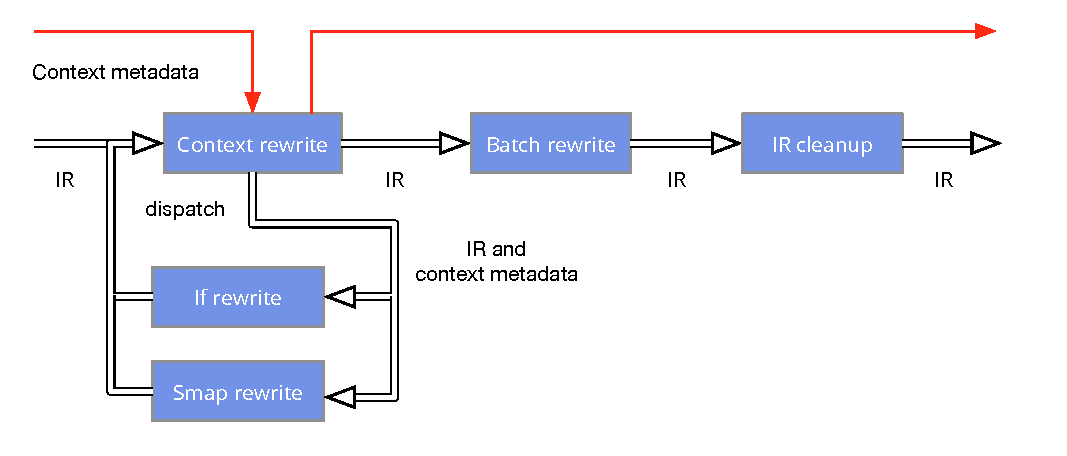
\includegraphics[width=\textwidth]{../Figures/yauhau-rewrite-flow}
    \caption{Rewrite order and flow in \yauhau{}}
    \label{fig:yauhau-rewrite-flow}
\end{figure}

You can see the full \yauhau{} transformation flow in Figure~\ref{fig:yauhau-rewrite-flow}.
We will discuss the individual parts of this flow graph in the upcoming sections.

\section{Runtime execution}

In \yauhau{} an accumulative fetch node, called \texttt{\_\_accum-fetch} statically replaces a set of fetches.
This is equivalent to a \textbf{round} in Haxl.
The accumulator is statically wired into the call sites of the fetches it replaces.
It has one input and one output for each \texttt{fetch} node it replaces.
Once a request for each input is present at runtime the accumulator executes, retrieving all of the requests simultaneously.

The parallel fetches are grouped into sequences of fetches on the same data source.
Each sequence is handed to its respective data source which has to perform the fetch.
In \yauhau{} this process is inherently parallel and each data source performs its request simultaneously.
In Haxl the programmer can choose whether to perform an asynchronous or synchronous request.
When all data sources are finished the results are distributed back through the corresponding outputs of the accumulator.
A visual representation of this can be seen in Figure~\ref{fig:yauhau-transformation}.

A new experimental and optional feature in \yauhau{} is to do dynamic dispatching of the finished requests.
This means once a certain data source returns with the data, computations only depending on that data source, can continue immediately.

\section{Data sources}

Similar to Haxl, compare Section~\ref{subs:datasources}, all data sources a user wants to access in \yauhau{} must be defined externally.

\yauhau{} has a more loose way of working with data sources than Haxl.
I/O actions in \yauhau{} are instances of the \texttt{Request} class.

\begin{figure}[h]
\begin{minted}{Java}
class Request<Payload, Return>{
  Paylod payload;
  IDataSource<Payload, Return> dataSource;
  Request(Payload payload,
          IDataSource<Payload, Return> dataSource)
    { /* implementation omitted */ }
  /* omitted code */
}
\end{minted}
\caption{Implementation of the \texttt{Request} class}
\label{fig:request-class-implementation}
\end{figure}

Each \texttt{Request} has two fields, an arbitrary Payload and a data source, compare Figure~\ref{fig:request-class-implementation} .
Here the data source, similarly to Haxl implements a Java interface \texttt{IDataSource}, see Figure~\ref{fig:idatasource-interface-implementation}, which provides a method for executing batched requests, hence the type \texttt{Iterable<Payload>} for the \texttt{fetch} method on the \texttt{IDataSource} interface (Figure~\ref{fig:idatasource-interface-implementation}   ).

\begin{figure}[h]
\begin{minted}{Java}
interface IDataSource<Payload, Return> {
  Object getIdentifier();
  Iterable<Return> fetch(Iterable<Payload> requests);
}
\end{minted}
\caption{Implementation of the \texttt{IDataSource} interface}
\label{fig:idatasource-interface-implementation}
\end{figure}

At runtime requests are grouped by the data source they are paired with and then handed to the respective source as a single sequence of many requests.

\section{Compile time transformation}

The basic \yauhau{} transformation, as mentioned, operates entirely on a dataflow graph.
The transformation does not concern itself with the kinds of nodes in the graph except for one, the \texttt{fetch} node/function which is a special node provided by the \yauhau{} library.
Beyond that, to simplify the transformation, it operates exclusively on the structure of the graph.
The \fetch{} node itself is implemented as a regular stateful function (See Figure~\ref{fig:fetch-implementation}) and works without the \yauhau{} transformation, although using it without the batching optimisation makes it much less useful.
Since data sources expect sequences of requests the \texttt{fetch} operator builds one and then returns the first element from the sequence of results returned by the data source.
If the source works as expected this result sequence should hold results of performing the requests in the same order as the requests were originally.

\begin{figure}[h]
\begin{minted}{Java}
class FetchOp<P, R> {
  @defsfn
  R fetch(Request<P, R> request) {
    List<P> l = Collections.singletonList(
                  request.getPayload()
                );
    Iterable<R> res = request.getDataSource().fetch(l);
    return res.iterator().next();
  }
}
\end{minted}
\caption{implementation of the \texttt{fetch} stateful function}
\label{fig:fetch-implementation}
\end{figure}

\subsection{Round detection}

The goal of the round detection is to find a minimal set of rounds.
A `round' is a set of \texttt{fetch} nodes with no data dependencies between the nodes.
Rounds must not overlap.
Hence the round detection finds a minimal set of non overlapping sets of data independent \texttt{fetch} nodes.

\subsubsection{Algorithm description}

To find the rounds in a given program I simulate the execution of the program and block code paths when a \texttt{fetch} node is encountered.
The simulation is done by topologically visiting the nodes of the graph while tracking three sets of items.

\begin{description}
	\item[created] The set of created bindings tracks which pieces of data that flow between the nodes of the program have been created prior to a particular point in the program.
	\item[visited] The set of visited nodes tracks which nodes were part of a previous stage.
	\item[round] The current round consists of all pending \fetch{} nodes.
	When a new fetch round is finalised it will consist of these \fetch{} nodes and the current round will be newly initialised empty.
\end{description}

Since bindings are unique in the dataflow IR we can track produced data by simply adding the respective binding to the set of created bindings.
The set of created bindings is initialised with the input parameters of our program.
From this point we traverse the graph in stages.
Each stage consists of the set of graph nodes where all inflowing data has previously been created and which was not in a previous stage.

For the former condition we check, for each input binding, whether the respective binding is contained in the set of \emph{created} bindings.
To ensure the latter condition a separate set of \emph{visited} nodes is maintained and only nodes which are not members of this set are allowed in a new stage.
Once the stage has been computed all functions in the stage are added to the \emph{visited} set.
Then all \fetch{} nodes are filtered from the stage and added to the current \emph{round}.
All remaining nodes are being executed.
Simulating to executing the nodes is done by simply adding all produced bindings (return bindings) of the node to the \emph{created} set.
If there are no remaining nodes to execute in a stage we have reached a point where the remainder of the dataflow graph depends on I/O actions, including the \fetch{} nodes.
Therefore the current round is maximal and we simulate executing all \texttt{fetch} nodes of the current round and dispatch a finalised fetch round.
Afterwards the current \emph{round} set is initialised empty again.
This is done until we get an empty stage, at which point we dispatch the current round again, unless it is empty, and we have reached the end of the round detection.

\begin{figure}
    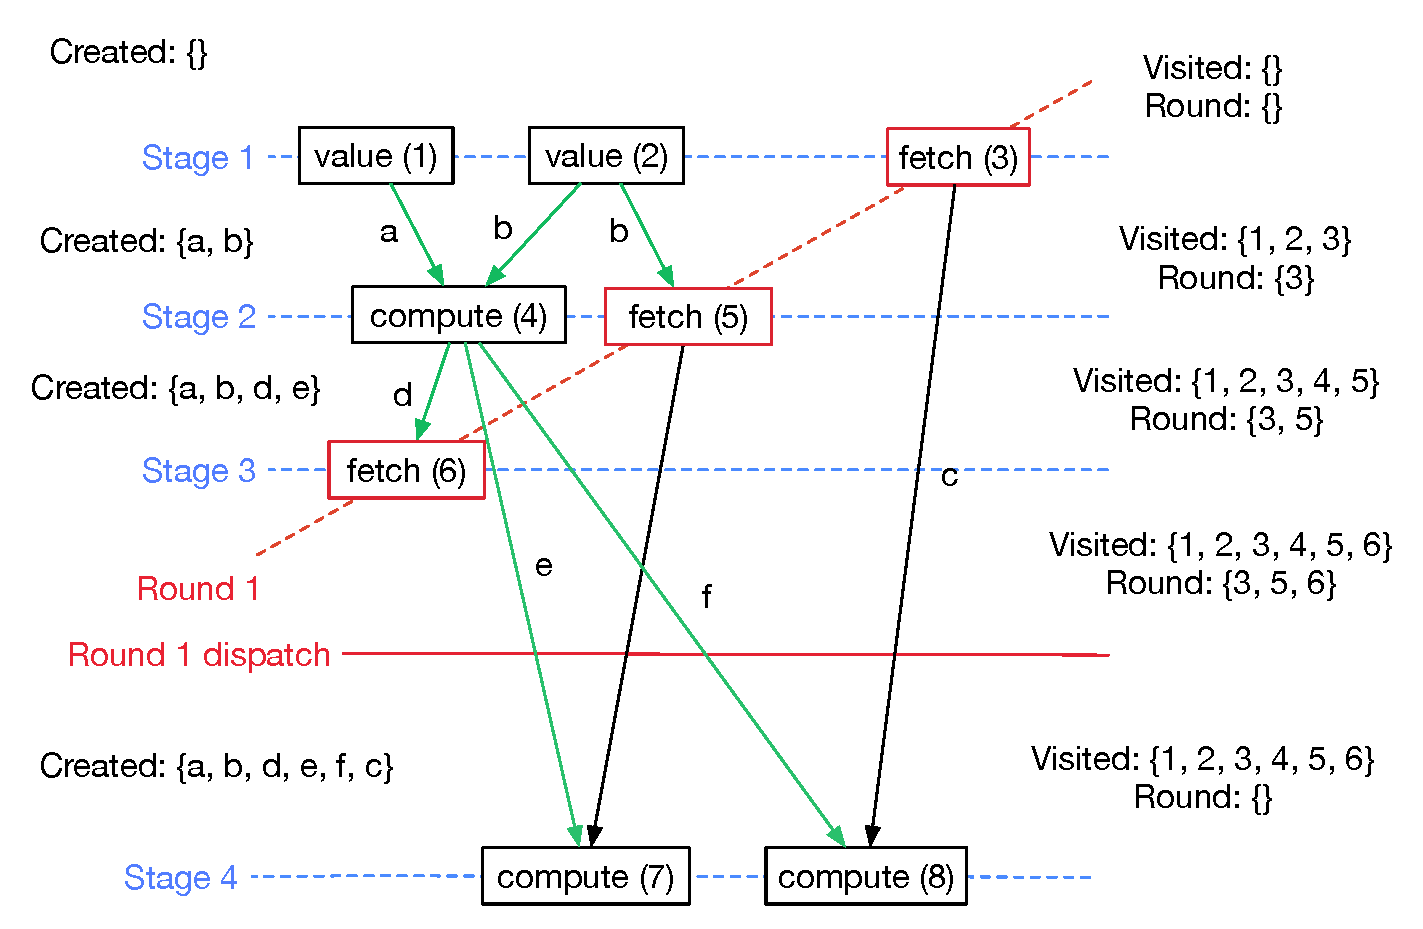
\includegraphics[width=\textwidth]{yauhau-round-detection}
    \caption{Example of the round detection algorithm}
    \label{fig:yauhau-round-detection}
\end{figure}

As an example you can see a typical dataflow IR graph in Figure~\ref{fig:yauhau-round-detection}.
The number after the node name is the unique id for that particular node and used for in the \emph{Visited} and \emph{Round} sets.
Blue dotted lines mark the stages as we traverse the graph.
In each stage only nodes for whom all incoming edges are created, symbolised, for up to the first round, by the green arrows, can be part of the stage.
You can also follow this algorithm along in Figure~\ref{fig:round-detection}.
After each stage the outgoing nodes are added to the created set as seen on the lefthand side.
The red \fetch{} nodes block the propagation through the graph and they are added to the \emph{Round} set on the righthand side.
After stage three we have no more nodes for whom all incoming edges are green, and therefore we dispatch a round of fetches, indicated by the dotted red line.
When the round has been dispatched, indicated by the solid red line, its created bindings are added to the \emph{Created}, visible after the dispatch on the lefthand side.

\begin{figure}
\textbf{Remarks:}
\begin{itemize}
  \item \texttt{set/union} is the set-union ($\cup$), \texttt{set/difference} is the set-difference ($\setminus$) and \texttt{\#\{\}} is an empty set.
  \item \texttt{filter} filters the collection where the predicate is true, \texttt{remove} where the predicate is false.
  \item \texttt{loop} and \texttt{recur} is tail recursion in clojure.
    \texttt{recur} restarts the body of \texttt{loop} with variables bound to the arguments of \texttt{recur}.
  \item \texttt{ir} is the ir graph give to the algorithm
\end{itemize}
\begin{minted}{Clojure}
(loop [visited #{}
       created #{}
       round #{}
       rounds []]
  (let [stage (set/difference
                (get-callable-fns created ir)
                visited)
        new-visited (set/union visited stage)]
    (if (empty? stage)
      ; end algorithm
      (if (empty? round)
        rounds
        (conj rounds round))
      ; continue
      (let [fetches (filter is-fetch? stage)
            non-fetches (remove is-fetch? stage)
            new-round (set/union round fetches)]
        (if (empty? non-fetches)
          ; dispatch round
          (recur new-visited
                 (set/union
                   created
                   (all-return-bindings new-round))
                 ; next round set to empty again
                 #{}
                 ; current round appended to rounds
                 (conj rounds new-round))
         ; continue to next stage
         (recur new-visited
                ; non-fetch bindings are now created
                (set/union
                  created
                  (all-return-bindings non-fetches))
                new-round
                rounds)))))
\end{minted}
\caption{Round detection algorithm in Clojure}
\label{fig:round-detection}
\end{figure}

\subsubsection{Result guarantees}

Adding the \fetch{} nodes to the set of visited nodes guarantees that rounds do not overlap.
Not simulating fetch execution before the round finishes guarantees that no round contains two fetches with data dependencies between them, since the dependent fetch would never have been in a stage before the round was finished since the required binding from the first fetch would not be created before the round finishes.
Finally since we only dispatch a round once no more executable nodes are found all other nodes have to be fully data dependent and this guarantees the set of rounds to be minimal.

\subsection{Graph rewrite}

Once the rounds have been computed an accumulated fetch is inserted for every round.
For each round all fetch nodes in the round are removed from the graph.
An accumulator is inserted with the combined inputs of all fetch nodes and the combined outputs of those nodes in the same order. See Figure \ref{fig:yauhau-transformation}.

\begin{figure}{h}
    \includegr{yauhau-transformation}
	\caption{Base transformation (taken from our paper\cite{ErtelGoensAdamEtAl2016})}
	\label{fig:yauhau-transformation}
\end{figure}

\subsection{Control flow considerations}

At runtime a node in the dataflow graph waits for inputs to arrive in channels.
There is one channel per function argument.
When the runtime scheduler activates the operator one input packet is removed from each channel and the stateful function is called with these arguments.
This process repeats until the scheduler decides to deactivate the node or if one of the input channels is empty.

These semantics are the same as they would be in a typical program, where every argument to a function has to be present for its call.
In dataflow this is not as straight forward as in typical code.
For instance free variables in algorithms inside an smap have to be specially handled during execution.
For clarification, smap is a mapping operation over a list.
It takes two arguments, an algorithm and a list of items and for each item in the list the algorithm is executed once with the item as argument collecting the results into a new list.
This is analogous to the \texttt{map} function in Haskell or Clojure, with the difference that there are some guarantees about execution order.
For a usage reference see Figure~\ref{fig:free-variables-in-smap}.

\begin{figure}
\begingroup
\definecolor{green(html/cssgreen)}{rgb}{0.0, 0.5, 0.0}
\catcode`\@=\active
\def@#1@{\textcolor{green(html/cssgreen)}{#1}}
\begin{minted}[escapeinside=||]{Clojure}
(ohua
  (let [free-var (add 4 5)
        list [1 2 3 4]]
    (smap
      (|@algo@| [item]
        (add item free-var))
      list)))
\end{minted}
\endgroup
\caption{Free variables in smap}
\label{fig:free-variables-in-smap}
\end{figure}

Normally variable bindings are simply translated into a set of arcs from where the value in the binding was created to each site where the variable is used.
When the source emits a value it is sent down each arc once.
This poses a problem in the case of smap where the target of the arc is a free variable inside the smap, like in Figure~\ref{fig:free-variables-in-smap}, and other inputs may receive many packets due to the mapping, whereas this input would naively only receive one.
What Ohua does to solve this is replicate sending the packet once for each element in the mapped collection.

In Yauhau we run into a similar problem.
We do not have free variables but perform an operation which is the complete opposite, where we rewrite connections to lead to an accumulator which is positioned outside the current control flow context (\texttt{smap}).
What we do not consider during our graph transformation is how often any of the fetch operators we are merging are called in the program.
If we have fetches in different contexts and naively accumulate them we create a similar situation to the one described above, where the inputs to the accumulator receive different amounts of data.
An example can be seen in Figure~\ref{fig:naive-batching-context-problem}.

In the example provided we can see two issues.
When a collection, which is longer than 1 is given to smap the respective input to the accumulator would be provided with a piece of data for each item in the collection whereas the bottommost input from \texttt{mk-req} would at the same time only receive a single piece of data.
At the same time the topmost two inputs comes from inside an if which means that only \textbf{one} of those two accumulator inputs would receive data during any execution of this program snippet, whereas the other receives nothing.

\begin{figure}
    \includegr{naive-transformation}
	\caption{Naive batching}
	\label{fig:naive-batching-context-problem}
\end{figure}

The structures which introduce issues like this are control flow structures, because they change how often or whether a particular section of code is executed.
Unfortunately the flow of control in a program is not structurally visible in our dataflow graph.
Therefore our accumulation transformation is unable to deal with this problem.

Instead of hammering support into this transformation I decided to add additional preparation steps before the batching transformation to produce an intermediate graph with certain properties such that the batching transformation is possible.
The properties of the graph we want are that any fetch in the same round is control flow wise in the same context, i.e. gets called the same amount of times.
Ensuring this particular property is easier if we simple pull every fetch out of any control flow context it is contained in so that it ends up being called exactly once in a given execution of the program.
Therefore our desired property of every fetch being executed the same amount of times holds and we can proceed with the transformation.

In the following Chapters I will explain how we handle \texttt{smap} (Chapter~\ref{ch:smap-transformation}) and \texttt{if} (Chapter~\ref{ch:if-transformation}) and how we generalise the two to define a pluggable, general transformation which ensures we handle nesting correctly (Chapter~\ref{ch:Context}).

% But first let me briefly explain the main idea behind those transformations.
